%%% XeLaTeX-article %%%
%# -*- coding: utf-8 -*-
%!TEX encoding = UTF-8 Unicode
%!TEX TS-program = xelatex  
%---------------------虽然加了%还是要保留!

\documentclass[17pt]{beamer}
\mode<presentation>
{
\usetheme[width=40pt]{Hannover}
\usecolortheme[]{dove}
\usefonttheme[]{structurebold}
\setbeameroption{hide notes}
}

\usepackage{fontspec}
\setmainfont{Arial} %设置主字体
\newfontfamily\sanskritfont[Script=Devanagari,Mapping=romantodevanagari,Scale=1.15]{Sanskrit 2003}             %输出天城体
%\newfontfamily\sanskritfont[Mapping=tex-text]{Times New Roman}              %输出转写
\doublehyphendemerits=-10000
\newcommand{\skt}[1]{{\sanskritfont{#1}}} %输出天城体
\newcommand{\skttrans}[1]{{\skt{#1}~#1}}  %输出天城体和转写
%----------------------------------------------------设置梵文输入方法 danda । ॥

\usepackage[UTF8,fontset=windows]{ctex}
\usepackage{amsmath}
%----------------------------------------------------设置中文环境

\usepackage{graphicx}
\usepackage{flafter} 
\graphicspath{{pic/}}
\usepackage{booktabs} 
\usepackage{nicematrix}
%-----------------------------------------插图表格

\usepackage{hyperref} 
\usepackage[dvipsnames]{xcolor}
\usepackage{colortbl}
\definecolor{light-gray}{gray}{0.9}
%------------------------------颜色

\newcommand{\verbroot}[1]{{$\sqrt{#1}$}}
\newcommand{\sktroot}[1]{{\verbroot{}\skt{#1}}}
\newcommand{\skttransroot}[1]{{\sktroot{#1}~#1}}
%---------------------------------------------------------------词根

\title{{梵语提高}}
\subtitle{2. 连声复习}
\author[张雪杉]{文学院~~张雪杉 \\ zhangxueshan@sdnu.edu.cn}
\date{}
%\institute{}


\begin{document}


\begin{frame}
  \titlepage
\end{frame}

\begin{frame}
  \frametitle{本节内容}
  \tableofcontents
\end{frame}

\section{连声总则}

\begin{frame}{\insertsection }
  \small
  \begin{itemize}
    \item 词间连声
    
    词与词之间,pada-ending
    \item 词内连声
    
    词根或词干与词缀之间
  \end{itemize}
\end{frame}

\section{词间连声}

\begin{frame}{落尾辅音}  
  \centering
  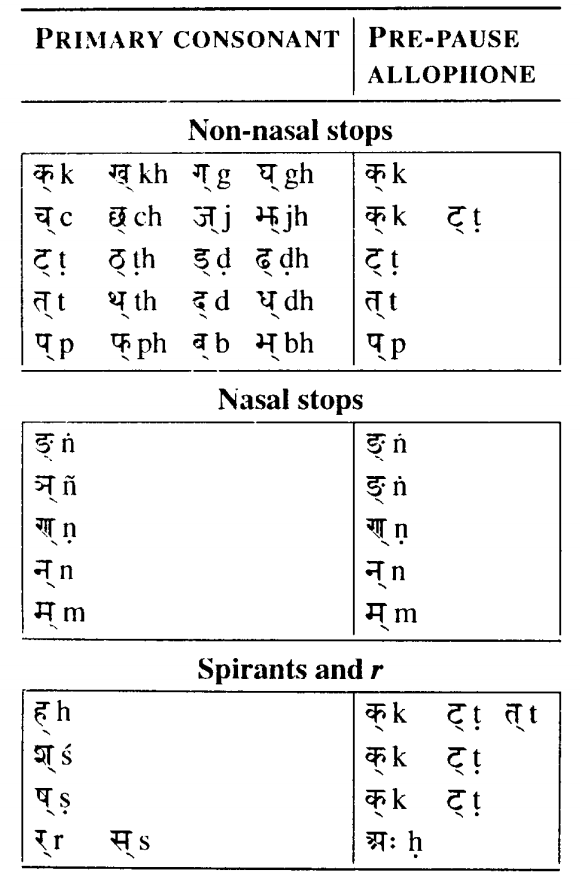
\includegraphics[width=0.5\textwidth]{consonantending.png} %
\end{frame}

\begin{frame}{元音连声}  
  \centering
  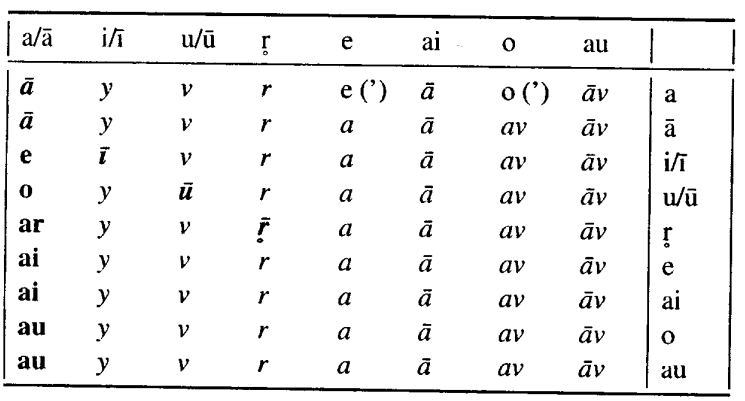
\includegraphics[width=0.9\textwidth]{vowelsandhi.png} %
\end{frame}

\begin{frame}{辅音和止音连声}  
  \centering
  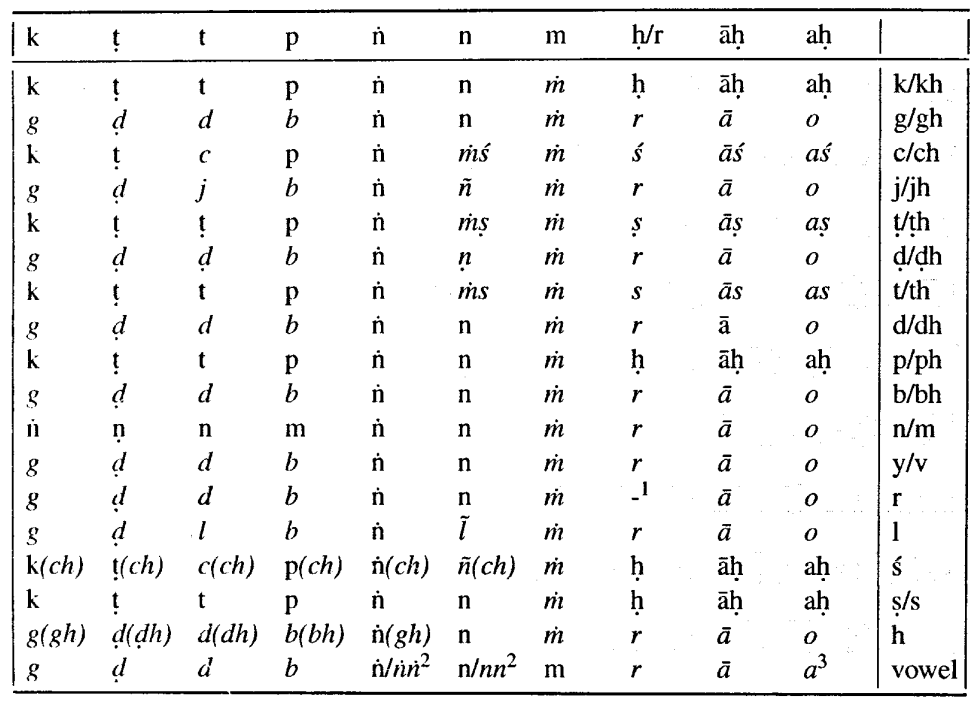
\includegraphics[width=\textwidth]{consonantsandhi.png} %
\end{frame}

\section{词内连声}

\begin{frame}{\insertsection ~~buddha连声}
  \begin{itemize}
    \item 送气浊音之后,t和th变成dh
    \item 浊辅音之前的辅音变成浊不送气
    \begin{itemize}
      \item \verbroot{}budh + ta = buddha
      \item \verbroot{}duh + ta = dugdha
      \item 反例:\verbroot{}dhā + thas(p2d) = dhatthaḥ
    \end{itemize}
  \end{itemize}
\end{frame}

\begin{frame}{\insertsection ~~ruki规则}
  \begin{itemize}
    \item 前音是非a/ā元音、半元音、h或者喉音时,s变成ṣ
    \item 前音和s中间插入了ṃ、ḥ或者咝音仍要变化
    \begin{itemize}
      \item agni + su = agniṣu
      \item yajuḥ + su = yajuḥṣu
      \item 反例:词尾不变 agnis tatra 
    \end{itemize}
  \end{itemize}
\end{frame}

\begin{frame}{\insertsection ~~n的顶化}
  \begin{itemize}
    \item 词内前方有ṛ、r或ṣ时,n变成ṇ
    \item 中间有元音、y、v、ṃ、ḥ、喉音和唇音仍要变化
    \begin{itemize}
      \item mitra(G.pl.) = mitrāṇām
      \item 反例:词尾不变 brahman, brahmaṇā
      \item 反例:ratha(I.sg.) = rathena 
    \end{itemize}
  \end{itemize}
\end{frame}



\section{下节预告}

\begin{frame}{\insertsection }
  \begin{itemize}
    \item
      第十八章复习
    
  \end{itemize}
\end{frame}  

\end{document}	
